\chapter{Flyweight模式}
\section{享元模式的概念}
\subsection{定义}
享元(Flyweight)模式的定义:运用共享技术来有効地支持大量细粒度对象的复用。它通过共享已经存在的又橡来大幅度减少需要创建的对象数量、避免大量相似类的开销,从而提高系统资源的利用率。
\par 通过尽量共享实例避免new出新实例。
\subsection{优点}
相同对象只要保存一份,这降低了系统中对象的数量,从而降低了系统中细粒度对象给内存带来的压力。
\subsection{缺点}
\begin{enumerate}
	\item 为了使对象可以共享,需要将一些不能共享的状态外部化,这将增加程序的复杂性。
	\item 读取享元模式的外部状态会使得运行时间稍微变长。
\end{enumerate}
\subsection{享元模式的角色}
享元模式有两种状态:
\begin{enumerate}
	\item 内部状态,即不会随着环境的改变而改变的可共享部分;
	\item 外部状态,指随环境改变而改变的不可以共享的部分。享元模式的实现要领就是区分应用中的这两种状态,并将外部状态外部化。
\end{enumerate}
享元模式的角色:
\begin{enumerate}
	\item Flyweight享元角色:是所有的具体享元类的基类,为具体享元规范需要实现的公共接口,非享元的外部状态以参数的形式通过方法传入。
	\item Concrete Flyweight具体享元角色:实现抽象享元角色中所规定的接口。
	\item Unsharable Flyweight非享元角色:是不可以共享的外部状态,它以参数的形式注入具体享元的相关方法中。
	\item Flyweight Factory享元工厂:负责创建和管理享元角色。当客户对象请求一个享元对象时,享元工厂检査系统中是否存在符合要求的享元对象,如果存在则提供给客户;如果不存在的话,则创建一个新的享元对象。
\end{enumerate}
\subsection{应用场景}
享元模式是通过减少内存中对象的数量来节省内存空间的,所以以下几种情形适合采用享元模式:
\begin{enumerate}
	\item 系统中存在大量相同或相似的对象,这些对象耗费大量的内存资源。
	\item 大部分的对象可以按照内部状态进行分组,且可将不同部分外部化,这样每一个组只需保存一个内部状态。
	\item 由于享元模式需要额外维护一个保存享元的数据结构,所以应当在有足够多的享元实例时才值得使用享元模式。
\end{enumerate}
\section{享元模式实现——例一}
\begin{table}[!h]
	\begin{tabular}{|l|l|}
		\hline
		名字&说明\\
		\hline
		BigChar&表示“大型字符”的类\\
		\hline
		BIgCharFactory&表示生成和共用BigChar类的实例的类\\
		\hline
		BigString&表示多个BigChar组成的“大型字符串”的类\\
		\hline
		Main&测试类\\
		\hline
	\end{tabular}
\end{table}
\begin{figure}[!h]
	\centering
	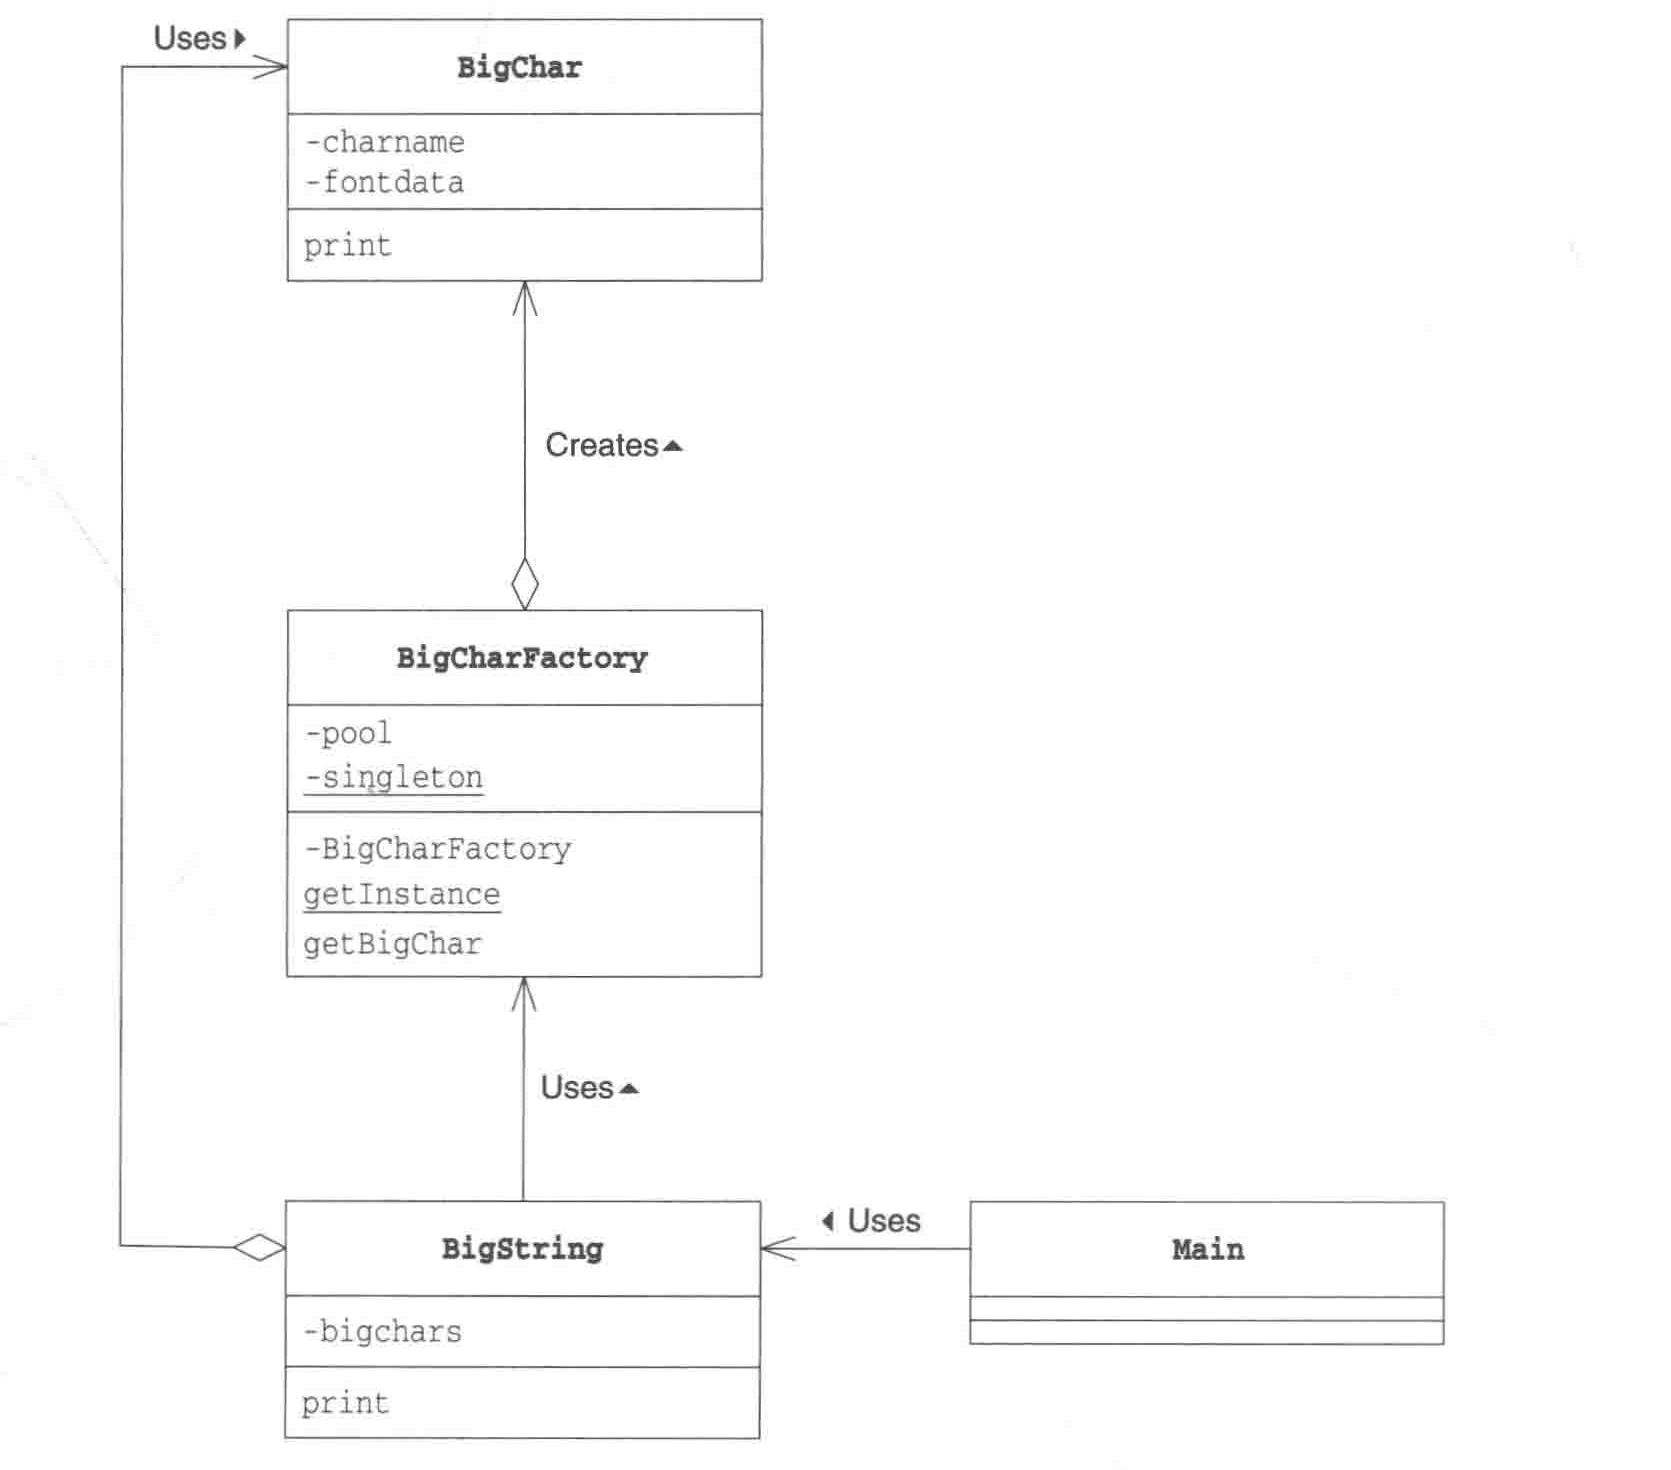
\includegraphics[width=\textwidth]{image/20-1}
	\caption{享元模式类图}
\end{figure}
\begin{lstlisting}
// 表示大型字符
public class BigChar {
	private char charName;
	//大型字符对应的字符串,由 # . \n 组成
	private String fontData;
	public BigChar(char charName) {
		this.charName = charName;
		try {
			BufferedReader reader = new BufferedReader(new FileReader("big" + charName + ".txt"));
			String line;
			StringBuffer buf = new StringBuffer();
			while ((line = reader.readLine()) != null) {
				buf.append(line);
				buf.append("\n");
			}
			reader.close();
			this.fontData = buf.toString();
		} catch (IOException e) {
			this.fontData = charName + "?";
		}
	}
	public void print() {
		System.out.println(fontData);
	}
}
\end{lstlisting}
\begin{lstlisting}
// 生成 BigChar 实例的工厂,实现了共享实例的功能。
public class BigCharFactory {
	// 管理已经生成的 BigChar 的实例
	private Map<String, BigChar> pool = new HashMap<>();
	private static BigCharFactory singleton = new BigCharFactory();
	
	private BigCharFactory() {}
	
	public static BigCharFactory getInstance() {
		return singleton;
	}
	
	public synchronized BigChar getBigChar(char charName) {
		BigChar bigChar = pool.get(charName);
		if (bigChar == null) {
			bigChar = new BigChar(charName);
			pool.put("" + charName, bigChar);
		}
		return bigChar;
	}
}
\end{lstlisting}
\begin{lstlisting}
// 由 BigChar 组成的字符串
public class BigString {
	// 大型字符的数组
	private BigChar[] bigChars;
	
	public BigString(String string) {
		this.bigChars = new BigChar[string.length()];
		BigCharFactory factory = BigCharFactory.getInstance();
		for (int i = 0; i < bigChars.length; i++) {
			bigChars[i] = factory.getBigChar(string.charAt(i));
		}
	}
	
	public void print() {
		for (int i = 0; i < bigChars.length; i++) {
			bigChars[i].print();
		}
	}
}
\end{lstlisting}
\begin{lstlisting}
public class Main {
	public static void main(String[] args) {
		BigString bigString = new BigString("12321");
		bigString.print();
	}
}
\end{lstlisting}
\section{享元模式实现——例二}
\begin{figure}[!h]
	\centering
	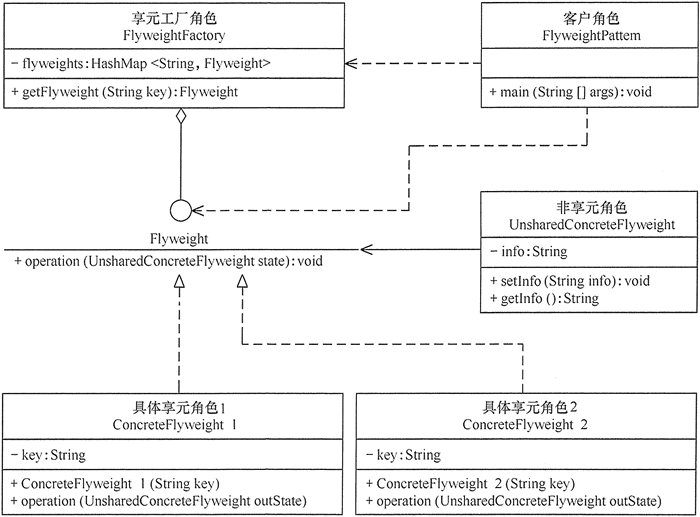
\includegraphics[width=0.9\textwidth]{image/20-2}
	\caption{享元模式的结构图}
\end{figure}
\begin{lstlisting}
//非享元角色
class UnsharedConcreteFlyweight {
	private String info;
	UnsharedConcreteFlyweight(String info) {
		this.info = info;
	}
	public String getInfo() {
		return info;
	}
	public void setInfo(String info) {
		this.info = info;
	}
}
\end{lstlisting}
\begin{lstlisting}
//抽象享元角色
interface Flyweight {
	public void operation(UnsharedConcreteFlyweight state);
}
//具体享元角色
class ConcreteFlyweight implements Flyweight {
	private String key;
	ConcreteFlyweight(String key) {
		this.key = key;
		System.out.println("具体享元" + key + "被创建!");
	}
	public void operation(UnsharedConcreteFlyweight outState) {
		System.out.print("具体享元" + key + "被调用,");
		System.out.println("非享元信息是:" + outState.getInfo());
	}
}
\end{lstlisting}
\begin{lstlisting}
//享元工厂角色
class FlyweightFactory {
	private HashMap<String, Flyweight> flyweights = new HashMap<String, Flyweight>();
	public Flyweight getFlyweight(String key) {
		Flyweight flyweight = (Flyweight) flyweights.get(key);
		if (flyweight != null) {
			System.out.println("具体享元" + key + "已经存在,被成功获取!");
		} else {
			flyweight = new ConcreteFlyweight(key);
			flyweights.put(key, flyweight);
		}
		return flyweight;
	}
}
\end{lstlisting}
\begin{lstlisting}
public class FlyweightPattern {
	public static void main(String[] args) {
		FlyweightFactory factory = new FlyweightFactory();
		Flyweight f01 = factory.getFlyweight("a");
		Flyweight f02 = factory.getFlyweight("a");
		Flyweight f03 = factory.getFlyweight("a");
		Flyweight f11 = factory.getFlyweight("b");
		Flyweight f12 = factory.getFlyweight("b");
		f01.operation(new UnsharedConcreteFlyweight("第1次调用a。"));
		f02.operation(new UnsharedConcreteFlyweight("第2次调用a。"));
		f03.operation(new UnsharedConcreteFlyweight("第3次调用a。"));
		f11.operation(new UnsharedConcreteFlyweight("第1次调用b。"));
		f12.operation(new UnsharedConcreteFlyweight("第2次调用b。"));
	}
}
\end{lstlisting}
\begin{lstlisting}
//output
具体享元a被创建!
具体享元a已经存在,被成功获取!
具体享元a已经存在,被成功获取!
具体享元b被创建!
具体享元b已经存在,被成功获取!
具体享元a被调用,非享元信息是:第1次调用a。
具体享元a被调用,非享元信息是:第2次调用a。
具体享元a被调用,非享元信息是:第3次调用a。
具体享元b被调用,非享元信息是:第1次调用b。
具体享元b被调用,非享元信息是:第2次调用b。
\end{lstlisting}
\section{模式扩展}
\subsection{单纯享元模式}
单纯享元模式,这种享元模式中的所有的具体享元类都是可以共享的,不存在非共享的具体享元类。
\begin{figure}[!h]
	\centering
	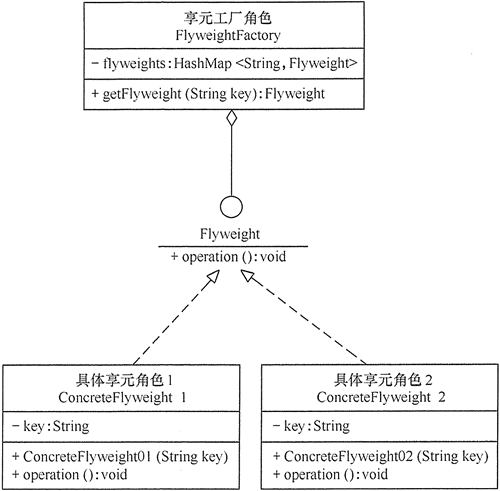
\includegraphics[width=0.6\textwidth]{image/20-3}
	\caption{单纯享元模式的结构图}
\end{figure}
\subsection{复合享元模式}
复合享元模式,这种享元模式中的有些享元对象是由一些单纯享元对象组合而成的,它们就是复合享元对象。虽然复合享元对象本身不能共享,但它们可以分解成单纯享元对象再被共享。
\begin{figure}[!h]
	\centering
	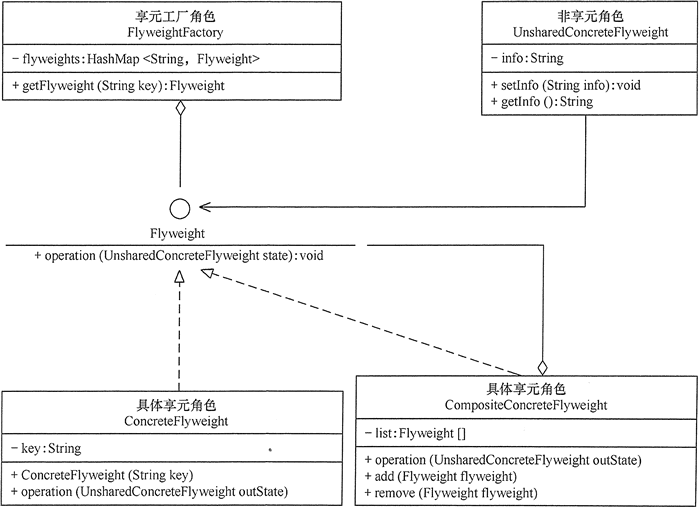
\includegraphics[width=0.8\textwidth]{image/20-4}
	\caption{复合享元模式的结构图}
\end{figure}
\section{思路扩展}
\begin{enumerate}
	\item 改变被共享对象,对多个地方产生影响。
	\item Intrinsic与Extrinsic
	\begin{itemize}
		\item Intrinsic应该被共享的信息,不依赖于位置与状况;
		\item Extrinsic不应该被共享的信息,依赖于位置与状况。
	\end{itemize}
	\item 注意不要让被共享的实例被垃圾回收器回收,显式回收只需要HashMap的remove即可。
	\item 内存之外的其他资源:文件句柄(文件描述符)和窗口句柄。
\end{enumerate}
\section{相关设计模式}
\begin{enumerate}
	\item Proxy模式:设置代理提高程序处理速度;
	而Flyweight针对节省生成实例资源。
	\item Composite模式:有时可以使用Flyweight共享Leaf角色。
	\item Singleton:Singleton只持有intrinsic信息。
\end{enumerate}
\section{思考}
\begin{enumerate}
	\item 获得程序内存使用量:
	\begin{lstlisting}
Runtime.getRuntime().gc();
long used = Runtime.getRuntime().totalMemory() - Runtime.getRuntime().freeMemory();
System.out.println("Used:" + used);
	\end{lstlisting}
	\item 例一中不使用synchronized问题:避免产生两个实例。
\end{enumerate}
